% % % % % % % % % % % % % % % % 
\section{Generalised Framework for an Ideal MRI Simulation System}
\label{chapterlabel4sec3}

This section of the survey focuses on introducing a generalised framework for an ideal MRI simulator to serve as a guideline for the MRI simulation community.
It is our belief that the proposed structure will aid in overcoming major limitations found throughout available simulators today and will also set the stage for my future work in my PhD project.
%Moreover, this framework can be used by the MR simulation community as a unifying guideline.
Our proposed framework is summarised in Figure~\ref{fig:globalFramework} and it is made up of 6 main components which will be explained next.

\hfill

\textbf{Solver.} At the heart of this framework is the \textbf{Bloch Equation Solver}, which independently solves the Bloch equation for each spin in the input object.
The \textbf{solver} is a highly parallelizable component of the framework which can run either on the computer's GPU or CPU and is based on the MRI simulator called POSSUM \cite{Drobnjak2006}.
The solver requires the following inputs:

\begin{itemize}
    \item \textbf{Sample Information}, such as:
    \textit{tissue specific parameters} (the nature of the nuclei, proton density, relaxation times and chemical shift), 
    \textit{geometry of the sample} (spin coordinates, resolution, total number of spins), and 
    \textit{motion trace} (translation and rotation values for each time point of the sequence).
    
    \item \textbf{Pulse Sequence Information}, such as:
    % \textit{Sequence Specific timings} (number of pulses in a multi-pulse sequence, repetition times and echo times),
    \textit{Radiofrequency Pulses} (amplitude and phase, duration, shape and timing), 
    \textit{Gradients} (shape, duration, timing) and
    \textit{Readout} (timing of each readout point).
    
    \item \textbf{Scanner Hardware Information}, such as:
    \textit{Main Magnet} (field strength, inhomogeneities in the main magnetic field),
    \textit{Gradient Limits} (maximum amplitude, slew rate) and
    \textit{Receiving/Transmitting Coils} (inhomogeneities in the coils, spatial sensitivity maps). 
\end{itemize}

\hfill

\textbf{Controllers.} The inputs described above are ubiquitous to any type of MRI simulation protocol.
However, our \textbf{Bloch equation solver} expects them in a certain format.
To overcome this limitation and to make our framework easily extensible, customisable and user friendly, we propose the existence of \textbf{Controllers}.
These are software wrappers which will translate user specific inputs into solver inputs.
With their help, the user can easily decide the complexity of the MRI simulation by choosing to include or exclude different sample specific, pulse sequence specific or hardware specific parameters.

\hfill

\textbf{Inputs.} The inputs to these controllers come in a variety of forms. 
For the sample object, the user can decide to either use a NIFTI phantom such as the \textit{BrainWeb digital brain phantom} \cite{Kwan1997}, or to create their own parameter maps consisting of the proton density, relaxation times and others.
If any of the required parameters are missing, a message will instruct the user about this error, while optional parameters will be omitted or set to some default values.

\hfill

For the pulse sequence, the user can decide to create their own sequence file consisting of timings ($T_R$, $T_E$), RF pulses ($N_{pulses}$, amplitude and phase), gradients (maximum amplitude, slew rate, shape) and readout timings, or they can use a scanner specific pulse sequence file.
%also choose to experiment with already created classic sequence such as gradient echo, echo planar imaging, etc, and only play with the
Finally, for the hardware configuration inputs, the user can choose to set the field strength ($B_0$) and the hardware limits for their simulation (maximum gradient amplitude, slew rate).
Additionally, for more complex scenarios, users can choose to include multi- transmit or receive coils with separate sensitivity maps or inhomogeneities in the coils.

\hfill

\textbf{GUIs. } Our framework also contains a set of \textbf{graphical user interfaces (GUIs)} which aid the end user in either rapidly prototyping new ideas or creating complex scenarios for MRI simulations.
Three GUIs are proposed: 
the \textit{Object GUI} for creating the input object and the motion trace,
the \textit{Pulse Sequence GUI} for creating the MRI pulse sequence and 
the \textit{Hardware Configuration GUI} for the hardware coil configuration.
The outputs from these GUIs become \textbf{inputs} for the software wrappers.

\hfill

\textbf{Reconstruction. } Having all of these in place, the \textbf{Bloch equation solver} will produce a set of signals corresponding to each coil used in the simulation.
These signals will be fed into a \textbf{reconstruction} block which, based on the type of readout used, can perform both Cartesian and non-Cartesian reconstructions.

\hfill

\textbf{Output. } The output of our proposed generalised framework is a set of reconstructed images and, if the option is enabled, the $x,y,z$ components of the magnetisation vector.
We have chosen to include the latter because in our experience with simulating MR sequences, we have found it to be very useful to have this extra piece of information available to you.

\hfill

Finally, it is our belief that this generalised framework can serve as a guideline for the MRI simulation community.
This is because it both provides a seamless interface between many required MRI modules and
it encourages the community to allow for integration of other open-source MR units.
For this reason, we also believe that it is important to develop this framework by using only open-source programming languages and packages.

\begin{figure}[ht]
    \centering
    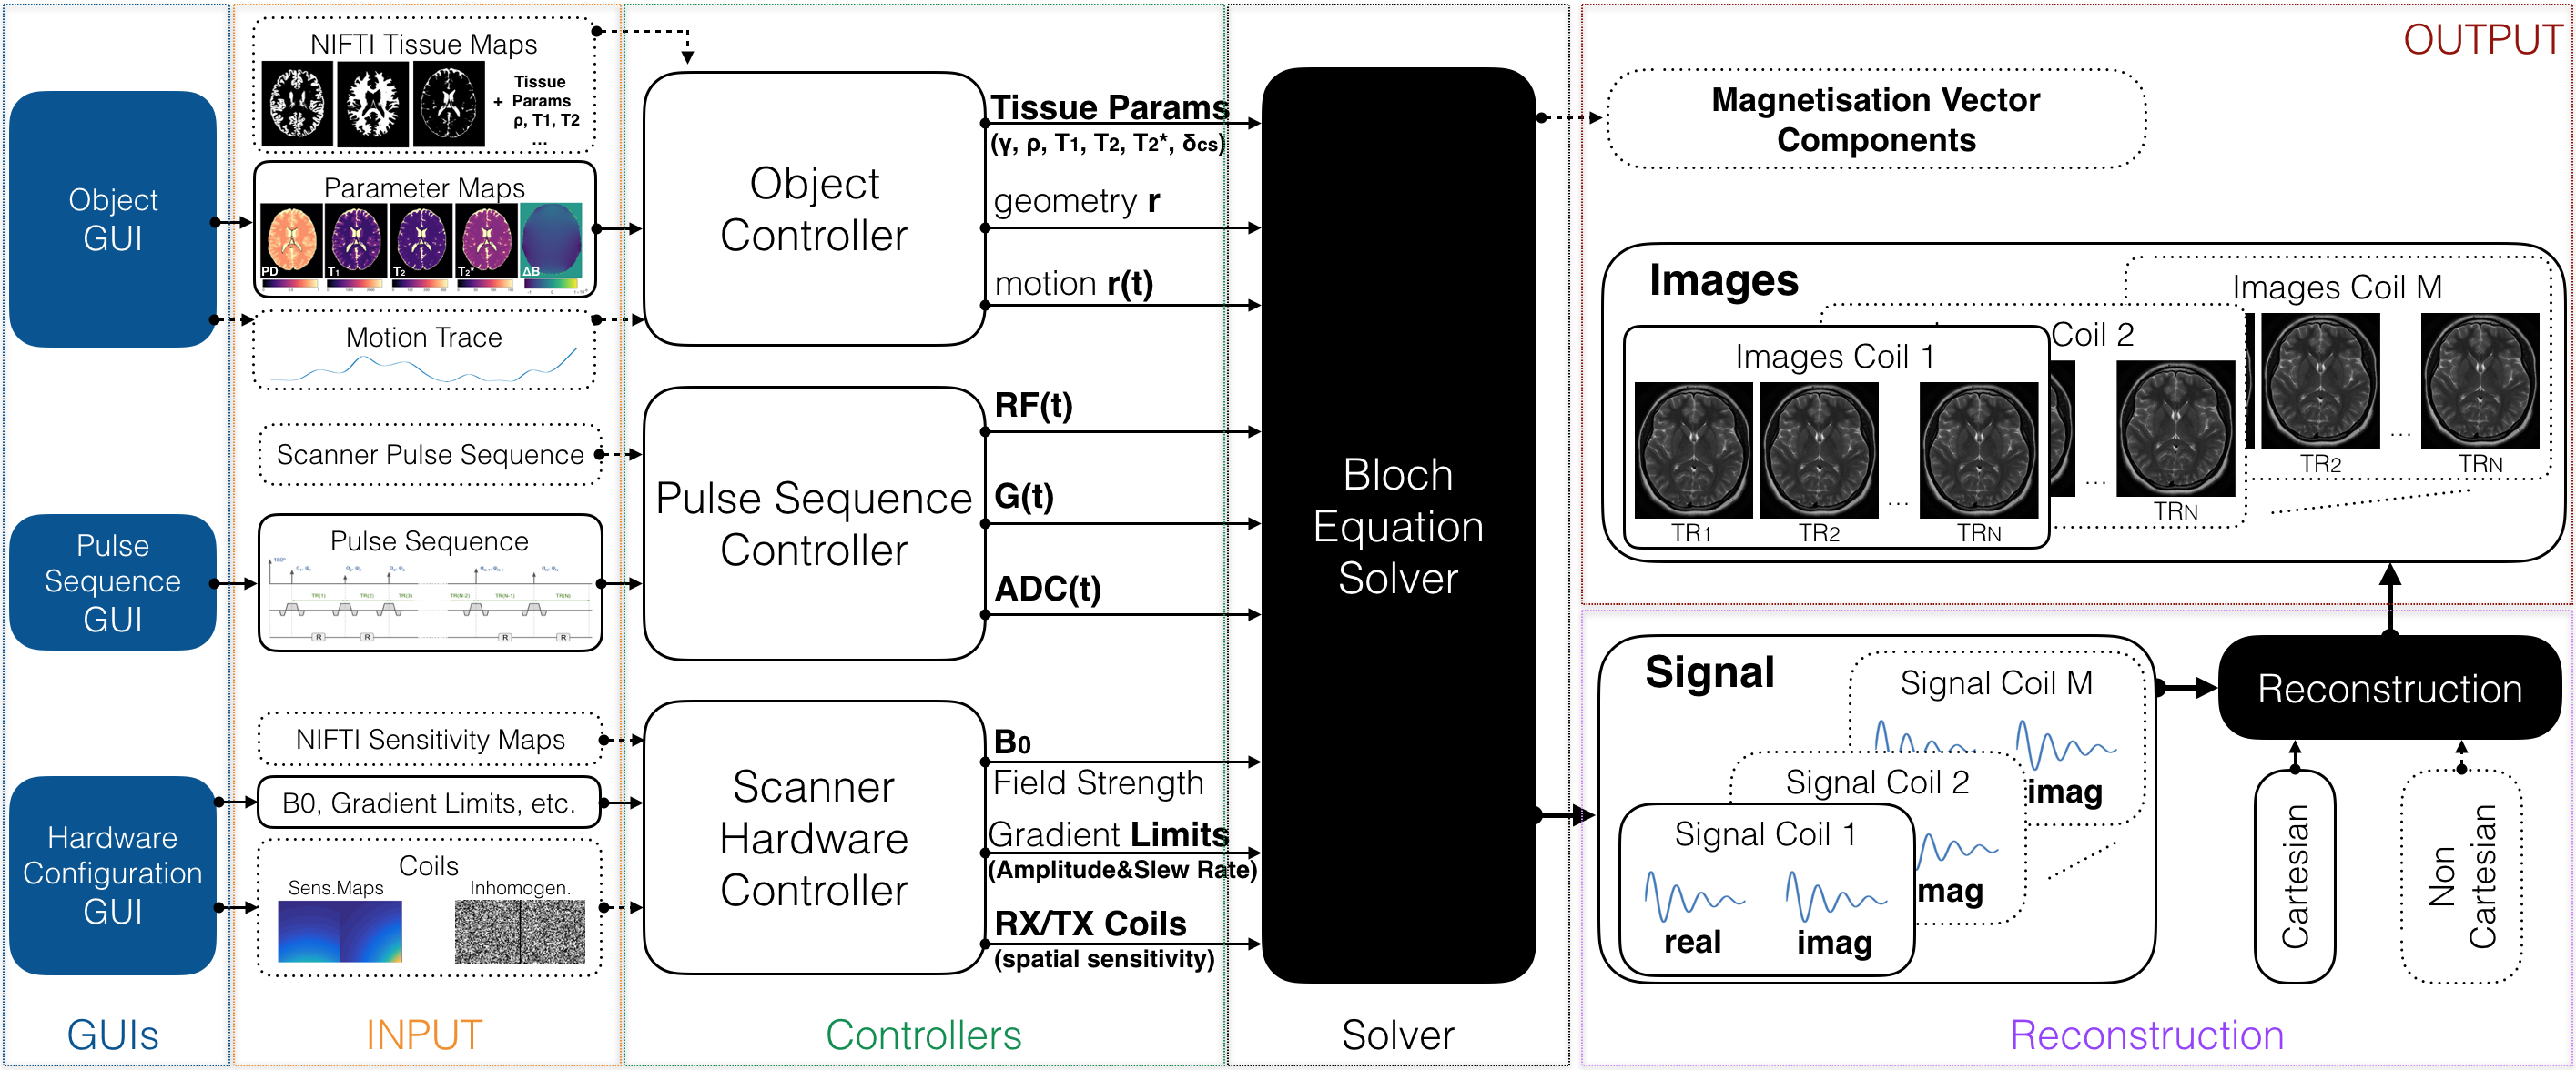
\includegraphics[angle=90,width=0.7\textwidth, keepaspectratio]{images/mri/globalFramework}
    \caption{Generalised framework for an ideal Magnetic Resonance Imaging simulator}
    \label{fig:globalFramework}
\end{figure}